% General Rules for the HuroCup humanoid robot competition
% The rules were initially created by Jacky Baltes and Thomas Braunl
% in 2002. 
% Jacky Baltes <jacky@cs.umanitoba.ca> 

\documentclass[12pt]{article}
\usepackage{graphicx}
%\usepackage{prelim2e}

%\usepackage[DVIps]{changebar}
% \setlength{\changebarsep}{3.5cm}

\newcommand{\HuroCup}{\textsc{HuroCup}}


\newcounter{law}[section]
\newcounter{comment}

\newcommand{\law}[2][Law]{ %
  \refstepcounter{law} %
  \renewcommand\thesubsection{#1-\arabic{law}} %
  \subsection{\hfill #2} %
}  

\newenvironment{lawlist}[1][Law]{ %
  \begin{enumerate} %
    \renewcommand{\theenumi}{#1-\arabic{law}.\arabic{enumi}}} %
  {\end{enumerate}}

\newenvironment{decisions}{\underline{\makebox[\textwidth][l]{\textbf{Decisions}}}\begin{enumerate}\renewcommand{\theenumi}{Dec-\arabic{law}.\arabic{enumi}}}{\end{enumerate}}

\newcommand{\comment}[1]{\refstepcounter{comment}
  \marginpar{C-\arabic{comment}} \textit{Comment-\arabic{comment}:#1}}

\begin{document}

\title{\HuroCup\\
  General Laws of the Game 2008}

\author{Jacky Baltes\\
Autonomous Agents Laboratory\\
University of Manitoba\\
Winnipeg, Manitoba\\
Canada, R3T 2N2\\
Email: jacky@cs.umanitoba.ca\\
WWW: http://www.cs.umanitoba.ca/\~{ }jacky\\[5mm]
Kuo-Yang Tu\\
National Kaohsiung First University of Science and Technology\\
Kaohsiung City, R. O. C.\\
Email: tuky@ccms.nkfust.edu.tw\\
}

\maketitle
\begin{abstract}
The following rules and regulations govern the game of \HuroCup, a
robotic game and robotics benchmark problem for humanoid
robots. 
%
\HuroCup\ attempts to encourage research into the many areas
of humanoid robotics, especially walking and balancing, complex motion
planning, and human robot interaction.
%
The \HuroCup\ competition also emphasizes the development of flexible,
robust, and versatile robots that can perform in many different
domains. 
%
In addition to the single events (e.g., sprint, penalty kick, obstacle
run, lift and carry, marathon, weight lifting, and basket ball), there
is an all-round competition for the single robot that performs best
over all events.
\end{abstract}

\section*{Latest Version of the Rules for \HuroCup}
\label{sec:updates}

The latest official version of the rules of the game for \HuroCup\ is
always available from the FIRA \HuroCup\ website (http://www.fira.net).

\newpage

\section{Mission Statement}

The goal of the \HuroCup\ league is to encourage research in
practical, autonomous, highly mobile, flexible, and versatile robotic
platforms. Intended applications for these robots are, among others,
search and rescue robots, care robots, etc.

As a benchmark problem, the goal of the \HuroCup\ league is to develop
humanoid robots that can perform several tasks in complex environments.

\section{Changes in the Laws of \HuroCup\ for 2008}

In many respects, 2007 was a new start for \HuroCup, and many things
changed. First and foremost, the old HuroSot name was changed to
\HuroCup\ to better reflect the large and complex events that sit at
the heart of \HuroCup.

2007 was the largest \HuroCup\ event ever with 20 teams participating
at the FIRA/RoboGames events in San Francisco. Furthermore, the
quality of the teams has greatly improved compared to previous years
and new world records were set at this event. The team from Tamkung
University in Taiwan managed to dethrone team Manus, from the National
University of Singapore, which had one the competition from 2003-2006.

The 2007 event also introduced several new events into the all-round
competition including weight lifting, marathon, and basketball. These
events were well received. Predictably, lift and carry and obstacle
run remained the most difficult events for the teams.

The aim of the rule changes for 2008 were to stabilize the competition
after the major changes that were introduced in the previous
year. Therefore, the introduction of the climbing wall competition was
delayed until 2009. 

Minor adjustments to the rules were made:
\begin{enumerate}
\item the robot dash event was renamed as the sprint event,
\item the robot must pick up a ball from a random position in front of it,
\end{enumerate}

I hope that we will have another exciting competition which will lead
to even more impressive research results and hope to welcome you all
in Qingdao, China.

\section{Physical Challenges}    
\label{sec:physical-challenges}

To reduce the steep learning curve toward fully autonomous humanoid
robots, the rules committee has developed seven challenges for
physical agents: (a) sprint, (b) penalty kick, (c) obstacle run, (d)
lift and carry, (e) weight lifting, (f) marathon, and (g)
basketball. These challenges are aimed at providing intermediate goals
on the path to fully autonomous robots that can operate in difficult
environments.

The following subsections describe each individual agent
challenge. These challenges are conducted using the FIFA Laws of the
Game (Section~\ref{sec:laws}) as much as possible. Unless otherwise
specified, the Laws of the Game apply.

\subsection{Sprint}
\label{subsec:sprint}

The sprint event (formerly named robot dash event) is a short distance
race for humanoid robots. The goal is for the robots to move as
quickly as possible from a start line to the end line for a series of
segments. For detailed rules of the robot sprint event, please refer to
the document titled ``\HuroCup\ Sprint - Laws of the Game.''

\subsection{Penalty Kick}
\label{subsec:penalty-kick}

In this event, the robot must approach and kick a ball positioned
somewhere in the ball area. A robot from a different team will act as
goal keeper during this event. For detailed rules of the penalty kick
event, please refer to the document titled ``\HuroCup\ Penalty
Kick - Laws of the Game.''

\subsection{Obstacle Run}
\label{subsec:obstacle-run} 

This event is similar to the sprint event
(Subsection~\ref{subsec:sprint}). The robot must move from one end of
the playing field to the other as quickly as possible. However, in
this case, a number of obstacles are distributed over the playing
field. The robot must navigate over, under, or around the obstacles
and reach the end zone. For detailed rules of the sprint event, please
refer to the document titled ``\HuroCup\ Obstacle Run - Laws of the
Game.''

\subsection{Lift and Carry}
\label{subsec:lift-and-carry}

The goal is to provide an event that requires robots to use active
balancing. The robots will be fitted with a small basket. The robots
repeatedly walk across an uneven terrain from one side to the
other. Once the robot reaches the end of the uneven terrain, the
referee adds small heavy obstacles into the basket. The robot must
compensate for the extra weight and continue to cross the uneven
terrain.  to walk. The robot that can carry the most weight is
declared the winner of the event. For detailed rules of the lift and
carry competition please refer to the document titled ``\HuroCup\ Lift
and Carry - Laws of the Game.''

\subsection{Marathon}
\label{subsec:marathon}

The marathon event is an endurance race over 42.195m. The robots
follow a coloured track. For detailed rules of the marathon event
please refer to the document titled ``\HuroCup\ Marathon - Laws of the
Game.''

\subsection{Weight Lifting}
\label{subsec:weight-lifting}

The goal of the weight lifting event is to develop robots that can
lift and balance heavy weights. For detailed rules of the weight
lifting event please refer to the document titled ``\HuroCup\ Weight
Lifting - Laws of the Game.''

\subsection{Basketball}
\label{subsec:basketball}

The basketball competition is another single robot event at the
moment, but wil be expanded to multiple players in the future. The
robot must throw a ball into a coloured target. For detailed rules of
the basketball event please refer to the document titled ``\HuroCup\
Basketball - Laws of the Game.''

\subsection{Soccer}
\label{subsec:soccer}

The soccer competition is the first team event in the \HuroCup\
competition. It is a game of soccer played by teams of 3 players. For
detailed rules of the lift and carry competition please refer to the
document titled ``\HuroCup\ Soccer - Laws of the Game.''

\section{Laws of the Game}
\label{sec:laws}

The following section describes the general law of the game for all
\HuroCup\  events. It is based on the FIRA rules as well as the FIFA
rules. 

\law{The Players}
\label{law:players}

\begin{lawlist}
\item \label{humanoid} The game is played using humanoid robots. The
  maximum size of the robots is 150cm. The maximum weight of the robot
  is 30 kg.
\item \label{categories} There are two categories of robots (small,
and large) depending on their height and the maximum foot
dimension. 

The \emph{height} of the robot is defined as the maximum distance
between any part of the robot and the ground when the robot is fully
extended.

The \emph{maximum foot dimension} is defined as the maximum
distance of any two points on any foot of the robot. Some
examples are shown in the Fig.~\ref{fig:foot-dimension}.

  \begin{figure}
    \begin{center}
      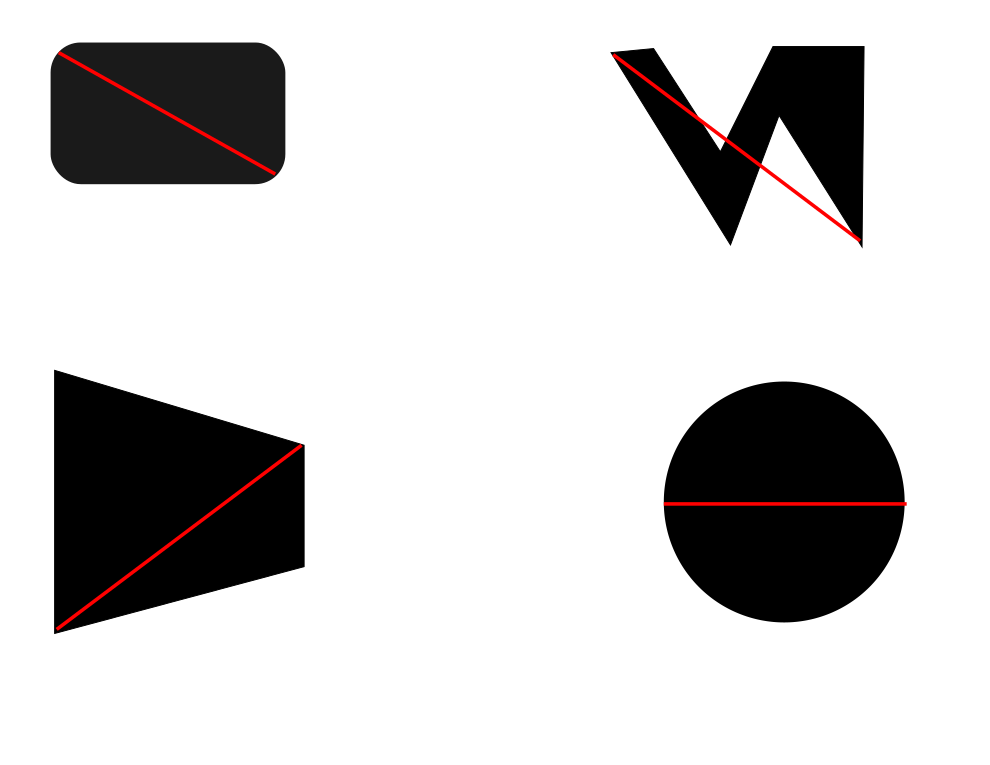
\includegraphics[width=0.7\textwidth]{Figures/foot-dimension}
    \end{center}
    \caption{Four examples of the maximum foot dimension for different
     robot feet.}
    \label{fig:foot-dimension}
  \end{figure}

  \begin{itemize}
    \item \emph{Small robots} are limited to a maximum height of 60cm
       and a maximum foot dimension of 13cm.
    \item \emph{Large robots} must have a height of more than 80cm and
    are limited to a maximum height of 150cm and a maximum foot
    dimension of 35cm.  
  \end{itemize}

\item \label{kinematics} The robot must be limited in its kinematics
to actions that could be performed with human kinematics.

\item \label{sensing} The sensors on the robot must be equivalent to
human sensors. 

\item \label{walking} The mode of locomotion of the robot must be
bipedal walking or running. 

\item \label{autonomous} Each robot must have the ability of fully
  independent locomotion, sensing, and processing. That is, all
  actuators, motors, power, computing, and sensing mechanisms must be
  incorporated into the robot.

\item \label{autonomous2} Each robot must be fully autonomous, that
  is, it must perform its own control decisions.

\item Before a game, each of the two teams has a color assigned,
  namely red or blue. Each team must be able to use either red
  or blue markers. The red team attacks the red goal and the
  blue team attacks the blue goal. 

\item Each robot must wear a team jersey with an assigned color
(red or blue). The team jerseys are small vests made out of light
material.

\item In addition, robots may use black and white coloring without
  restriction. Other colors may be used so long as they are deemed by
  the rules committee to be sufficiently different from reserved
  colors, specifically ball yellow, marker red and
  marker blue.

\item A robot must not have in its construction anything that is
  dangerous to itself, another robot, human operators, or spectators.

\item For any infringement of this Law:
  \begin{itemize}
  \item play must be stopped,
  \item the offending robot as identified by the referee has to be
    removed from the playing field,
  \item the robot may be repaired and the fault identified by the
    referee may be corrected,
  \item the repaired robot may not re-enter the field without the
    referee's permission,
  \item the referee checks that the fault has been repaired before
    allowing the robot to re-enter the field,
  \item the robot may only re-enter the field if the ball is out of
    play. 
  \end{itemize}
\end{lawlist}

\begin{decisions}
\item The local organizing committee should make examples of possible
  vests available to the participants as soon as possible.

\item The height of the robot includes all appendages such as sponsor
  markings, ornaments, antennas.
  
\item The features of robots that are forbidden under~\ref{kinematics}
  are special kicking devices on the foot, spinning upper bodies, or
  feet that can kick at a 90 degree angle.

\item In 2009, the restriction on the sensors of the robot will be
  strictly enforced. In particular, a robot is not allowed to use
  sonar or infra-red sensors.

\end{decisions}

\law{The Referee}
\label{law:referee}

\begin{lawlist}

\item Every match is controlled by a referee who has full authority to
  enforce the Laws of the Game in connection with the match to which
  he has been appointed.

\item The referee
  \begin{enumerate}
    \item enforces the Laws of the Game,
    \item controls the match possibly in co-operation with the
      assistant referee,
    \item ensures that any ball used meets the requirements of
      the laws of the game,
    \item ensures that the robotic equipment meets the requirements of
      Law~\ref{law:players},
    \item stops, suspends or terminates the match, at his discretion,
      for any infringements of the Laws,
    \item stops, suspends or terminates the match because of outside
      interference of any kind,
    \item stops the match if, in his opinion, a robot is likely to
      cause serious harm to humans, other robots or itself and ensures
      that it is removed from the field of play,
    \item repositions the ball to a neutral position if it becomes
      stuck during play,
    \item punishes the more serious offense when a robot commits more
      than one offense at the same time,
    \item takes disciplinary action against robots guilty of
      cautionable and sending-off offenses. He is not obliged to take
      this action immediately but must do so when the ball next goes
      out of play,
    \item acts on the advice of assistant referees regarding incidents
      which he has not seen,
    \item ensures that no unauthorized persons enter the field of play,
    \item restarts the match after it has been stopped,
    \item provides the appropriate authorities with a match report
      which includes information on any disciplinary action taken
      against team officials and any other incidents which occurred
      before, during or after the match,
    \item allows play to continue when the team against which an
      offense has been committed will benefit from such an advantage
      and penalizes the original offense if the anticipated advantage
      does not ensue at that time,
    \item takes action against team officials who fail to conduct
      themselves in a responsible manner and may at his discretion,
      expel them from the field of play and its immediate surrounds.
  \end{enumerate}

\item The decisions of the referee regarding facts connected with play
  are final.

\item The referee may only change a decision on realizing that it is
  incorrect or, at his discretion, on the advice of an assistant
  referee, provided that he has not restarted play.

\item A referee (or where applicable, an assistant referee) is not
  held liable for: 
  \begin{enumerate}
    \item kind of injury suffered by an official or spectator,
    \item any damage to property of any kind,
    \item any other loss suffered by any individual, club, company,
      association or other body, which is due or which may be due to
      any decision which he may take under the terms of the Laws of
      the Game or in respect of the normal procedures required to
      hold, play and control a match.

      This may include:

      \begin{itemize}
      \item a decision that the condition of the field of play or its
        surrounds are such as to allow or not to allow a match to take
        place,
      \item a decision to abandon a match for whatever reason,
      \item a decision as to the condition of the fixtures or
        equipment used during a match including the field and the ball,
      \item a decision to stop or not to stop a match due to spectator
        interference or any problem in the spectator area,
      \item a decision to stop or not to stop play to allow a damaged
        robot to be removed from the field of play for repair,
      \item a decision to request or insist that a damaged robot be
        removed from the field of play for repair,
      \item a decision to allow or not to allow a robot to have
        certain colors,
      \item a decision (in so far as this may be his responsibility)
        to allow or not to allow any persons (including team or
        stadium officials, security officers, photographers or other
        media representatives) to be present in the vicinity of the
        field of play,
      \item any other decision which he may take in accordance with
        the Laws of the Game or in conformity with his duties under
        the terms of the FIRA Federation or league rules or
        regulations under which the match is played.
      \end{itemize}
    \end{enumerate}
\end{lawlist}
                                
\law{The Assistant Referee}
\label{law:assistant-referee}

\begin{lawlist}
\item The assistant referee is appointed whose duties, subject to
  the decision of the referee, are to 
  \begin{enumerate}
  \item act as timekeeper and keep a record of the match
  \item monitor the robot operators for illegal signals being sent
    to the robots
  \item indicate when an interchange is requested
  \item indicate when misconduct or any other incident has
    occurred out of the view of the referee
  \item indicate when offenses have been committed whenever the
    assistants are closer to the action than the referee (this
    includes, in particular circumstances, offenses committed in
    the penalty area)
  \item indicate whether, at penalty kicks, the goalkeeper has
    moved forward before the ball has been kicked and if the ball
    has crossed the line
  \end{enumerate}
  
\item The assistant referees also assist the referee to control
  the match in accordance with the Laws of the Game. In the event
  of undue interference or improper conduct, the referee will
  relieve an assistant referee of his duties and make a report to
  the appropriate authorities.
\end{lawlist}


\end{document}


% *** Local Variables: ***
% *** mode: LaTeX ***
% *** mode: outline-minor ***
% *** mode: auto-fill ***
% *** outline-regexp: "% !\\|\\\\\\(sub\\)*section" ***
% *** TeX-command-default: "LaTeX PDF" ***
% *** End: ***
